\documentclass[11pt]{article}

\usepackage{graphicx}
\usepackage[hidelinks]{hyperref}

\title{Software Engineering notes}
\author{Matteo Salvino}
\date{}

\begin{document}
\maketitle
\pagebreak
\tableofcontents
\pagebreak
\section{Capability Maturity Model Integration}
Now days companies want to deliver products and services better, faster and cheaper. At the same
time, in the high-technology environment of the twenty-first century, nearly all organizations have found themselves building increasingly complex products and services. It's unusual today for a single organization to develop all the components that compose a complex product or service. More commonly, some components are built in-house and some are acquired; then all the components are integrated into the final product or service. Organizations must be able to manage and control this complex development and maintenance process. The problems these organizations address today involve enterprise-wide solutions that require an integrated approach. Effective management of organizational assets is critical to business success. In other words, these organizations are product and service developers that need a way to manage their development activities as part of achieving their business objectives. In the current marketplace, maturity models, standard, methodologies and guidelines exist that can help an organization to improve the way it does business. However, most available improvement approaches focus on a specific part of the business and do not take a systematic approach to the problems that most organizations are facing. So, focusing on improving one particular business area, these models are hindered by barriers that exist in organizations. \textbf{CMMI} for development (CMMI-DEV) provides an opportunity to avoid or eliminate these barriers. It consists of best practices that address development activities applied to products and services. It address practices that cover the product's lifecycle from conception through delivery and maintenance. The goal is to build and maintain the total product. CMMI-DEV contains 22 process areas. Of those process areas, 16 are core process areas, 1 is a shared process area and 5 are development specific process areas. The Software Engineering Institute (SEI) in its research, has found some key points on which organizations can focus on to improve its business.
\begin{center}
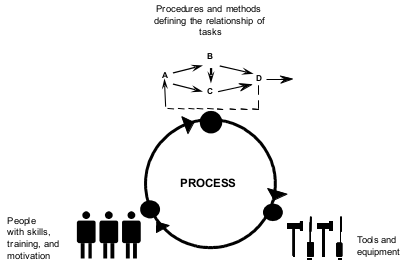
\includegraphics[scale=0.40]{./images/SEI_key_points.png}
\end{center}
In particular these key points are : people, procedures and methods, and tools and equipment. These points are kept together by the processes used in our organization. They allow us to address scalability and provide a way to incorporate knowledge of how to do things better. Processes allow us to leverage our resources and to examine business trends. We are focusing on methodologies, not because people and technologies aren't important, but since the technology changes at an incredible speed and people can works for different companies, in this way we can provides the infrastructure and stability necessary to deal with an ever-changing world and to maximize the productivity of people and the use of technology to be competitive. The SEI has taken the process management premise "the quality of a system of product is highly influenced by the quality of the process used to develop and maintain it" and defined CMMs that embody this premise. A CMM, including CMMI, is a simplified representation of the world, which contains the essential elements of effective processes. CMMs focus on improving processes in an organization, describing an evolutionary path from an immature process to disciplined mature process with improved quality and effectiveness. CMMI can be used in process improvements also as a framework, which provides the structure needed to produce CMMI models, training and evaluation components. To allow the use of multiple models withing the CMMI framework, model components are classified as either common to all CMMI models or applicable to a specific model. The common material is called \textbf{CMMI Model Foundation} (CMF). The components of the CMF are part of every model generated from the CMMI framework. Those components are combined with material applicable to an area of interest to produce a model. A \textbf{constellation} is defined as a collection of CMMI components that are used to construct models, training materials and evaluate related documents for an area of interest. CMMI-DEV previously introduced is the development constellation for a model. All CMMI models contains multiple \textbf{Process Areas} (PAs). A process area is a cluster of related practices in an area that, when implemented collectively, satisfies a set of goals considered important from making improvement in that area. Some of these area are : Causal Analysis and Resolution (CAR), Configuration Management (CM), etc. We can define two type of goal :
\begin{itemize}
\item \textbf{Generic} : it's called generic because the same goal statement applies to multiple process areas. A generic goal describes the characteristics that must be present to institutionalize processes that implement a process area. It's a required model component and is used in evaluation to determine whether a process area is satisfied or not. The istitutionalization is an important concept in process improvement, since it implies that the process in ingrained in the way the work is performed and there is a commitment and consistency to performing the process. The progress of process institutionalization is characterized by the type of the generic goal :
\begin{itemize}
\item \textbf{GG1 \- Performed process} : a performed process is a process that accomplishes the work necessary to satisfy the specific goals of a process area.
\item \textbf{GG2 \- Managed process} : a managed process is a performed process that is planned and executed in accordance with some policy. It employs skilled people having adequate resources to produce controlled outputs. It's controlled, monitored, reviewed and evaluated for adherence to its process description. The process can be instantiated by a project, group or organizational function. Management of the process is concerned with institutionalization and the achievement of other specific objectives established for the process, such as cost, schedule and quality objectives. The control provided by a managed process helps to ensure that the established process is retained during times of stress. The requirements and objectives for the process are established by the organization. The status of the work products and services are visible to management at defined points. Commitments are established among those who perform the work and the relevant stakeholders and are revised as necessary. Work products are reviewed with relevant stakeholders and are controlled. A critical distinction between a performed process and a managed process is the extent to which the process is managed. A managed process is planned and its execution is managed against the plan. Corrective actions are taken when the actual results and execution deviate significantly from the plan. A managed process achieves the objectives of the plan and is institutionalized for consistent execution. 
\item \textbf{GG3 \- Defined process} : a defined process is a managed process that is tailored from the organization's set of standard processes according to the organization's tailoring guidelines. It has a maintained process description and contributes process related experiences to the organizational process assets. Organizational process assets are artifacts that relate to describing, implementing and improving processes. These artifacts are assets because they are developed or acquired to meet the business objectives of the organization and they represent investments by the organization that are expected to provide current and future business value. The organization's set of standard processes, which are the basis of the defined process, are established and improved over time. Standard processes describe the fundamental process elements that are expected in the defined processes. Standard processes also describe the relationships among these process elements. A project's defined process provides a basis for planning, performing and improving the project's task and activities. A critical distinction between a managed process and a defined process is the scope of application of the process descriptions, standards and procedures. For a managed process, the process descriptions, standards and procedures are applicable to a a particular project, group or organizational function. As a result, the managed processes of two projects in one organization can be different. Another critical distinction is that a defined process is described in more detail and is performed more rigorously than a managed process. Finally, management of the defined process is based on the additional insight provided by an understanding of the interrelationships of the process activities and detailed measures of the process, its work products, and its services.
\end{itemize}
\item \textbf{Specific} : a specific goal describe the unique characteristics that must be present to satisfy the process area. It's a required model component and is used in evaluation to determine whether a process area is satisfied or not.
\end{itemize}
\subsection{Understanding levels}
Levels are used in CMMI-DEV to describe an evolutionary path recommended for an organization that wants to improve the processes it uses to develop products or services. CMMI supports two improvement paths using levels. One path enables organizations to incrementally improve processes corresponding to an individual process area selected by the organization. The other path enables organizations to improve a set of related processes by incrementally addressing successive sets of process areas. These two improvement paths are associated with the two types of levels : \textbf{capability levels} and \textbf{maturity levels}. These levels correspond to two approaches to process improvement called \textbf{representations}. In turn, the two representations are called \textbf{continuous} and \textbf{staged}. Both representations provide ways to improve our processes to achieve business objective and use the same model components. The continuous representation is concerned with selecting both a particular process area to improve and the desired capability level for that process area. The staged representation is concerned with selecting multiple process areas to improve within a maturity level. Both capability levels and maturity levels provide a way to improve the processes of an organization and measure how well organizations can and do improve their processes. However, the associated approach to process improvement is different.
\subsubsection{Capability levels (Continuous representation)}
To support those who use the continuous representation, all CMMI models reflect capability levels in their design and content. The four capability levels, each of them is a layer for the process improvement, are designated by the numbers 0 through 3 :
\begin{itemize}
\item \textbf{0. Incomplete} : an incomplete process is a process that either is not performed or is partially performed. One or more of the specific goals of the process area are not satisfied and no generic goals exist for this level since there is no reason to institutionalize a partially performed process.
\item \textbf{1. Performed} : a performed process is a process that accomplish the needed work to produce work products; the specific goals of the process area are satisfied.
\item \textbf{2. Managed} : a managed process is a performed process that is planned and executed in accordance with some policy; It employs skilled people having adequate resource to produce controlled outputs; it involves relevant stakeholders; It's monitored, controlled, reviewed and evaluated for adherence to its process description. The process discipline reflected by capability level 2 helps to ensure that existing practices are retained during times of stress.
\item \textbf{3. Defined} : a defined process is a managed process that is tailored from the organization's set of standard processes according to the organization's tailoring guidelines and contributes work products, measures, and other process improvement information to the organizational process assets.
\end{itemize}
\subsubsection{Maturity levels (Staged representation)}
To support those who use the staged representation, all CMMI models reflect maturity levels in their design and content. A maturity level is a defined evolutionary plateau for organizational process improvement. Each maturity level matures an important subset of the organization's processes, preparing it to move to the next maturity level. The maturity levels are measured by the achievement of the specific and generic goals associated with each predefined set of process areas. The five maturity levels are designated by the numbers 1 through 5 :
\begin{itemize}
\item \textbf{1. Initial} : in this layer processes are usually ad hoc and chaotic. In spite of this chaos, maturity level 1 organizations often produce products and services that work, but they frequently exceed the budget and schedule documented in their plans. These organizations are characterized by a tendency to overcommit, abandon their processes in a time of crisis, and be unable to repeat their successes.
\item \textbf{2. Managed} : as before.
\item \textbf{3. Defined} : as before.
\item \textbf{4. Quantitatively managed} : it's a defined process that is controlled using statistical and other quantitative techniques. Quantitative objectives for quality and process performance are established and used as criteria in managing the process. Quality and process performance is understood in statistical terms and is managed throughout the life of the process.
\item \textbf{5. Optimizing} : it's a quantitatively managed process that is improved based on understanding of the common causes of variation inherent in the process. The focus of an optimizing process is on continually improving the range of process performance through both incremental and innovative improvements.
\end{itemize}
\subsection{ISO family}
\textbf{ISO 12207} defines and structures all activities involved in the software development process. Its main goal is to provide a common language to involved stakeholders. It's based on a functional approach : a set of coordinated activities transforming an input in an output. It's based on two basic principles :
\begin{itemize}
\item \textbf{Modularity} : it means processes with minimum coupling and maximum cohesion.
\item \textbf{Responsibility} : it means to establish a responsibility for each process, in order to facilitate the application of the standards in a project where there are many people involved.
\end{itemize}
\textbf{ISO 9000} is maintained by ISO and is administered by accreditation and certification bodies. This family of ISO addresses "Quality management". Its fundamental building blocks are :
\begin{itemize}
\item \textbf{Quality management system} : it deals with general and documentation requirements that are the foundation of the management system. In particular, the previous requirements can be explained in details :
\begin{itemize}
\item \textbf{General} : they are general requirements like how the processes of the management system interact to each other or how you will measure and monitor the processes.
\item \textbf{For documentation} : they are requirement focused on the documentation. They can require what documentation is needed to operate the system effectively or how it should be controlled.
\end{itemize}
\item \textbf{Management responsibility} : it manage high level responsibilities like set policies and objectives or plan how the objectives will be met.
\item \textbf{Resource management} : it deals with the people and physical resources needed to carry out the process. People should be competent to carry out their task and physical resources and work environment need to be capable of ensuring that the customer's requirements are satisfied.
\item \textbf{Product-service realization} : it deals with the processes necessary to produce the product or to provide the service.
\item \textbf{Measurement, analysis, and improvement} : it deals with measurements to enable the system to be monitored. For example we can measure if the processes are effective or if the product really satisfy customer's requirements.
\end{itemize}
ISO doesn't itself certify organizations. There are accreditation bodies that authorize certification bodies. Organizations can apply for ISO 9001 compliance certification to a certification body. The various accreditation bodies have mutual agreements with each other to ensure that certificates issued by one of the Accredited Certification Bodies (CB) are accepted worldwide. An ISO certificate is not a once-and-for-all award, but must be renewed at regular intervals recommended by the certification body, usually around three years. \textbf{Quality requirements} are a set of process requirements and resources that constitute the Quality Manual (QM) of the organization. This latter specifies the organization's quality policy regardless specific commitments and customers. It's adapted to specific projects, generating several Quality Policies (QP). The ISO 9001 certification required that processes are described in the two previous specific documents (QM and QP).
\section{Software Development Process Models}
Software products are not tangible. In order to manage a software project the project manager needs special methods. So, the monitoring process in based on the explicit definition of activities to be performed and documents to be produced. These documents allow us to monitor the progress of the process and give us an idea of its quality. Software Development Process Models and their instances, differ from each other for the required activities and for the produced documents. Now, we will see several software process models, discussing their pros and cons.
\subsection{Waterfall model}
A Waterfall model is a typical process in which there are separate and distinct phases of specification and development. So, first we describe all the specifications of the software and then we have a subsequent phase that take care about the development. Its main phases are :
\begin{itemize}
\item \textbf{Requirements analysis and definition}
\item \textbf{System and software design}
\item \textbf{Implementation and unit testing}
\item \textbf{Integration and system testing}
\item \textbf{Operation and maintenance}.
\end{itemize}
Each phase depends on the deliverables of the previous one and corresponds to a specialization of tasks. One of its main drawback is the difficulty of allows changes after the process in started. Another drawback is that the end users doesn't have a vision of the overall system (uncertainty). So, they have to wait till a working version of the system is available. In turn, programmers have to wait the analysis phase before starting their job. The solution is to use an iterative approach.
\subsection{Process iteration}
The system requirements always evolve during the project development, so process iteration where earlier stages are reworked is always part of the process for large systems. Iteration can be applied to any of the generic process models. Typically, an iteration follows one of the following approaches :
\begin{itemize}
\item \textbf{Incremental delivery} : we start building a small system (prototype) and next we enlarge it (incremental way). A \textbf{prototypal model} is constituted by a customer interaction in order to obtain customer's requirements, then we build a prototype also called \textbf{mock-up}  (when we build a system with feels and looks similar to the final system, but without working software behind), and then we present it to the user, in order that he is able to test the prototype and say "Ok, i'm satisfied", or viceversa. If the answer is positive, then we can start to implement the functionality behind the mockup. The \textbf{incremental model} is formed by iterations which are constituted by analysis, design, implementation and test phases. The result of a generic iteration $i$ typically is the system with version $i$. It's very similar to the prototypal model but in this case the intermediate version are full working and it allows for a more accurate design. Its main drawback is that if we figure out a wrong functionality in a specific system version, we have to throw away a lot of job previously done, whereas in the first model we will build only the mock-up system. In the incremental development we define the requirements, then we assign each of them to a specific system release version, design the whole system architecture, then develop, validate and integrate the system increment, and finally validate the system. If this isn't the last iteration, then we continue to increment the functionality of our system, otherwise we have built the final system. In other words, delivering part of the required functionality. Then the user requirements are prioritized and the highest priority requirements are included in early increments (early versions). Once the development of an increment is started, the requirements are frozen though requirements for later increments can continue to evolve. The trade off is the length of these iterations, the bigger the interval is then we move towards the waterfall model, the smaller the interval is then will be more difficult to build a very good software architecture. Its advantages are the following : the customer can see at each iteration an increment of the system functionalities, early increments act as a prototype to help asking requirement for future iterations, lower risk of overall project failure and the highest priority system requirements tends to receive the most testing.
\item \textbf{Spiral development} : in spiral development the process is represented as spiral (rather than a sequence) of activities. Each loop in the spiral represents a phase in the process. There not exist fixed phases such as specification or design (the loops in the spiral are chosen depending on what is required). The risks are explicitly evaluated and resolved throughout the process. In particular, the spiral model is constituted by the following sectors :
\begin{itemize}
\item \textbf{Objective setting} : they are specific objectives for the current phase.
\item \textbf{Risk assessment and reduction} : the risks are evaluated and activities punt in place to reduce the key risks.
\item \textbf{Development and validation} : in this sector we choose a development model for the system.
\item \textbf{Planning} : the project is reviewed and the next phase of the spiral is planned.
\end{itemize}
\end{itemize}
\subsection{Formal methods}
Formal methods are formalisms based on logic or algebra for requirement specification, development and test. They don't use the natural language, because it's very ambiguous, but tends to write the specification of the software in some formal languages like Z, Z++, etc.
\subsection{Extreme programming}
It's a part of the Agile model family. It's an approach based on the development and delivery of very small increments of functionality. It relies on constant code improvement, use involvement in the development team and pairwise programming.
\subsection{Core process activities}
Now, lets quickly review the main activities involved in the development process :
\begin{itemize}
\item \textbf{Software specification} : it's the process of establishing what services are required and the constraints on the system operations and development. These requirements can be functional or non-functional (they regards about system quality). This process is also called requirements engineering process. First of all it perform a feasibility study to understand if building the system is feasible. Typically this phase produce a document called feasibility report. Subsequently, the requirements are defined, analyzed and validated. The results of these phases constitute the so called requirement document.
\item \textbf{Software design and implementation} : it's the process of converting the system specification into an executable system. The software design phase is a process that in which we design the software structure (architectural, component, data structures, etc.) that fulfill the specifications. In the implementation phase we translate the previous structure into an executable program. In this phase our goal is also to remove as many errors as possible from the program generated, typically using a program testing. These two phases are closely related and may be interleaved. 
\item \textbf{Software validation} : the verification and validation is intended to show that the system is conform to its specifications (verification) and meets the customer's requirements (validation). Typically the system is tested over test cases that are derived from the specification of the real data to be processed by the system. We can use several types of testing :
\begin{itemize}
\item \textbf{Unit test} : individual components are tested independently.
\item \textbf{System test} : test the whole system.
\item \textbf{Acceptance test} : testing with customer data to check that the system meets the customer's needs.
\end{itemize}
\item \textbf{Software evolution} : software is very flexible and can change over time. A change of the requirements must be reflected also in the software.
\end{itemize}
\end{document}